\section{Fragment Centros y Sitios de Interés}
El objetivo de este fragment es mostrar un mapa al usuario de manera que este pueda interactuar con los elementos, asi como poder conocer su ubicación a tiempo real y obtener información de los centros e instalaciones de la UGR así como de sitios que puedan ser de interés general

El motivo de que ambos fragments se traten de manera conjunta es que en cuanto a implementación se refiere ambos estan inmplementados en el proyecto de la misma manera.

Estos fragments funcionan en base al fragment de \textbf{Google Maps}. Utilizamos una clave API solicitada a google para poder acceder a las funcionalidades basicas de los mapas.

Hacemos uso de la ubicación del usuario --- después de previamente solicitar los permisos necesarios --- para mostrar la ubicación de este a tiempo real en un mapa. Tambien utilizamos el \textbf{sensor} de brújula para permitir orientar el mapa según la orientiación fisica del usuario.

El mapa que se muestra en el fragment de centros es un mapa personalizado de google que la ugr pone a disposición de los usuarios con toda la información sobre sus centro y diversas instalaciones.

El mapa utilizado en el fragment sitios de interés se trata de un mapa de google que contiene marcadores en sitios turisticos y de interes general para cualquier persona que visite o desee conocer la ciudad

A continación pasaremos a detallar la implementación de ambos fragments

\subsection{Variables}

\begin{itemize}
	\item gestorPosicion
	\item callback
\end{itemize}

La primera variable \textbf{gestorPosicion} simplemente se encarga de crear una instancia de la clase gestor de posición que resumidamente es la que se encarga de gestionar todos los procesos y rutinas que tienen que ver con la ubicación del usuario.

La variable \textbf{callback} contiene sin embargo una fución. Dicha función se ejecutara una vez el mapa haya sido cargado y este listo para ser usado. Esta función se encarga de crear un mapa y centrar la ubicación en la posción del usuario en caso de tener los permisos de ubiciación o en una localización por defecto en caso de no tener dichos permisos. Finalmente carga el archivo que contiene los datos del mapa.

\newpage

\subsection{Métodos}
Los métodos implementados por estos fragments son:

\begin{itemize}
	\item onCreate
	\item onOptionsItemSelected
	\item onCreateOptionsMenu
	\item onLocationChanged
	\item onCreateView
	\item onViewCreated
\end{itemize}

\subsubsection{onCreate}
El método onCreate simplemente llama al método onCreate superior de la clase fragment y utiliza
\begin{lstlisting}[language=Kotlin]
setHasOptionsMenu(true)
\end{lstlisting}
para activar la opción de que el fragment tenga un menu de opciones para poder activar o desactivar el sensor de brújula.

\subsubsection{onOptionsItemSelected}
Este método se encarga de activar la brújula una vez se marca el item y de desactivarla si se encuentra activad. Resumidamente conmuta el estado del sensor de brújula.

\subsubsection{onCreateOptionsMenu}
Este método se encarga de crear el menu que permite activar y desactivar la brújula.

\subsubsection{onLocationChanged}
Este método se encarga de llamar a la función del gestor de posición:

\begin{lstlisting}[language=Kotlin]
gestorPosicion.actualizarPosActual(requireContext(), requireActivity(), it)
\end{lstlisting}

cuando detecta un cambio en la ubicación del usuario, lo que permite mantener la misma actualizada a tiempo real.

\subsubsection{onCreateView}
El método onCreateView simplemente se encarga de cargar el fragment de \textbf{Google maps}.

\subsubsection{onViewCreated}
Este método es el que se encarga de solicitar los permisos haciendo uso de la función:

\begin{lstlisting}[language=Kotlin]
GestorPermisos.getLocationPermission(requireContext(), requireActivity())]
\end{lstlisting}

Y además se encarga de llamar a la función que almacena la variable \textbf{callback}:

\begin{lstlisting}[language=Kotlin]
mapFragment?.getMapAsync(callback)
\end{lstlisting}

\begin{figure}[H]
\begin{subfigure}{0.5\textwidth}
  \centering
  % include first image
  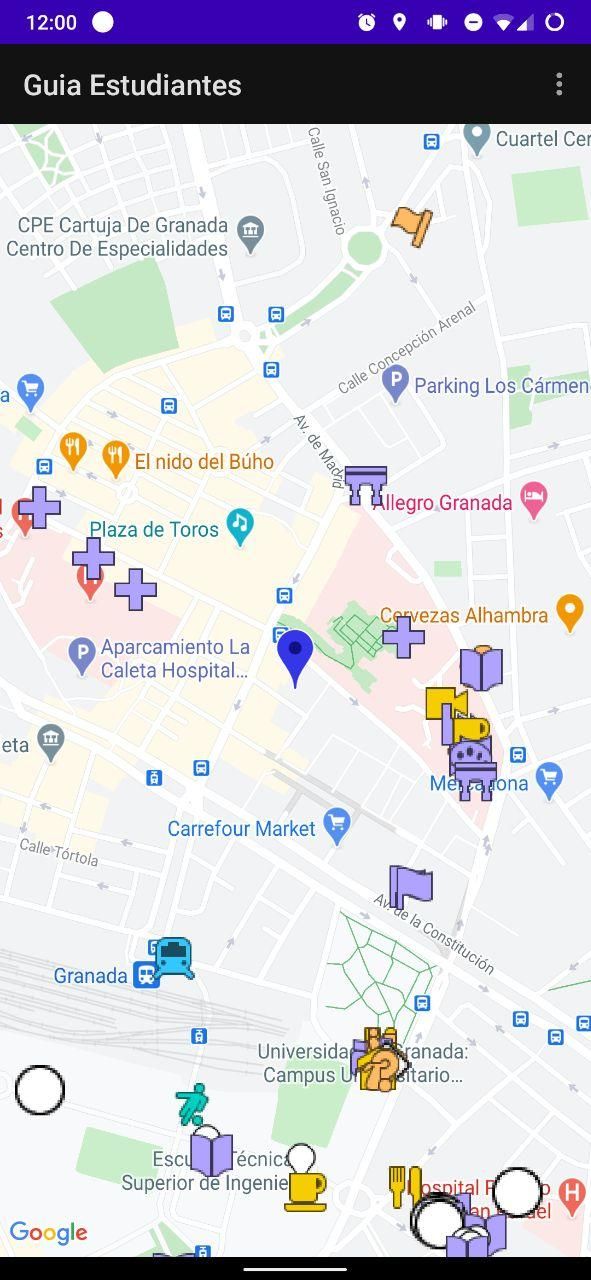
\includegraphics[width=1\linewidth]{centros}
  \caption{Centros}
  \label{fig:sub-first}
\end{subfigure}
\begin{subfigure}{0.5\textwidth}
  \centering
  % include second image
  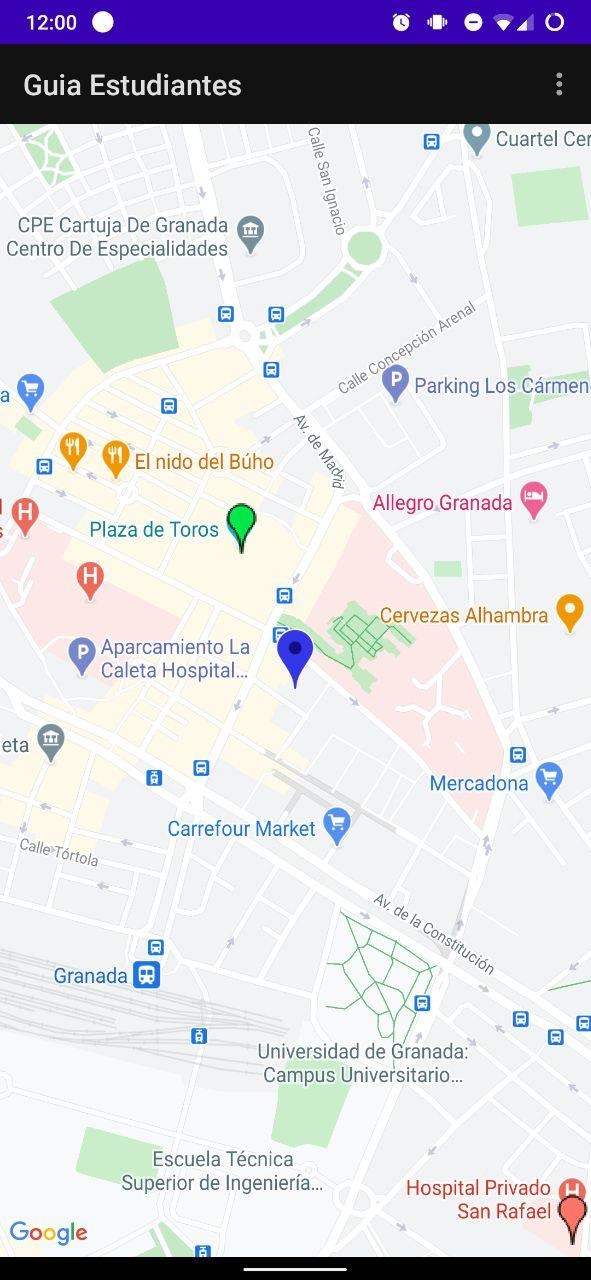
\includegraphics[width=1\linewidth]{sitiosinteres.jpg}
  \caption{Sitios de interes}
  \label{fig:sub-second}
\end{subfigure}
\end{figure}

